\section{不确定性分析}\label{sec:uncertainty}

\begin{chapterquestion}
\textbf{本章研究的问题}：如何度量代理模型预测的可信程度？
\end{chapterquestion}

\subsection{基于深度集成的不确定性估计}

第~\ref{sec:anomaly}~节的过度外推现象表明：仅输出单点预测 $\hat y$ 的代理，
无法评估预测的可信程度。为此需要模型同时输出预测的确定性程度。
本文采用深度集成（DeepEnsemble）：训练 $M=3$ 个结构相同、
仅初始化种子与数据 shuffle 不同的 MLP，对任意输入给出
\begin{equation}
    \mu(x)=\frac{1}{M}\sum_{m=1}^{M}\hat f_m(x),\qquad
    \sigma(x)=\sqrt{\frac{1}{M-1}\sum_{m=1}^{M}\big(\hat f_m(x)-\mu(x)\big)^2}.
\end{equation}
$\mu(x)$ 是预测均值（与单模型同等精度，$R^2=0.9995$），
$\sigma(x)$ 是成员间的预测分歧，度量的不是数据噪声，
而是模型对该输入的认知不确定性：在数据充分覆盖处成员预测趋于一致（$\sigma$ 小），
在训练数据稀疏/分布外处成员间预测分歧较大（$\sigma$ 大）。

\begin{figure}[H]
\centering
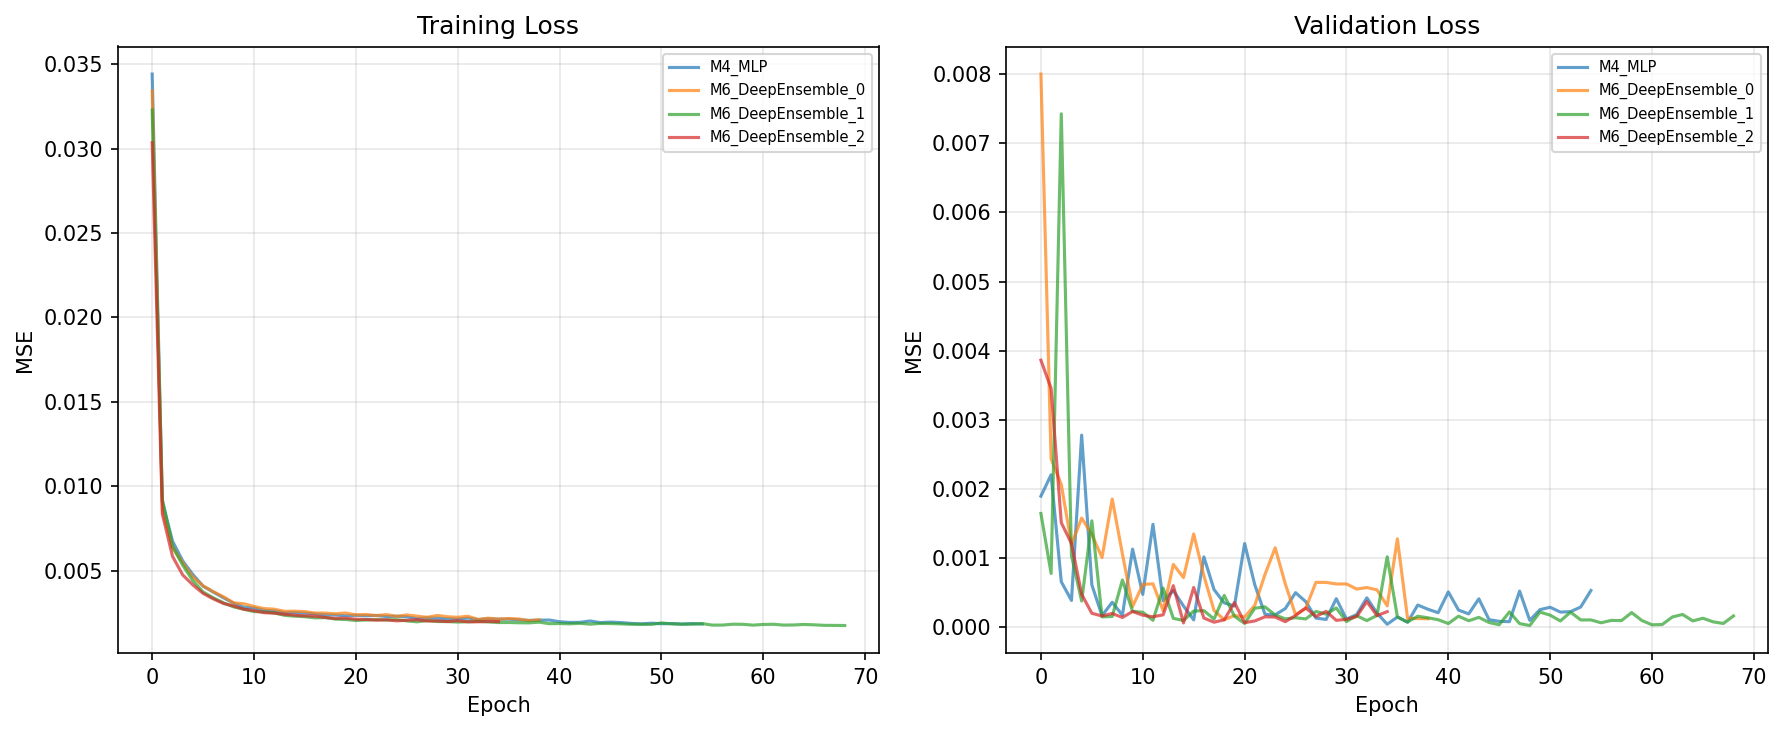
\includegraphics[width=0.78\textwidth]{figures/04_loss_curves.png}
\caption{神经网络/集成成员的训练-验证损失曲线（Early Stopping 约 200 轮触发）}
\label{fig:loss}
\end{figure}

\subsection{研究目标的转向}

引入 $\sigma(x)$ 后，研究目标由"预测是否准确"转向"预测是否可信"：
\begin{itemize}
    \item \textbf{高分解是否落在高不确定区域？}\quad
        第~\ref{sec:anomaly}~节中 $\mu>100$ 的过度外推解，正是 $\sigma(x)$ 显著偏大的位置；
        模型的高预测值与高不确定性同时出现，构成可检测的风险信号。
    \item \textbf{高分解是否落在低密度区域？}\quad
        以训练集近邻距离度量数据密度，过度外推的高预测值往往出现在样本稀疏的极端工况
        （如下压力远超训练上界），即代理缺乏证据支撑的区域。
\end{itemize}

即 $\sigma(x)$ 显式标记了代理在何处可信、在何处不可信。
这将第~\ref{sec:anomaly}~节的定性问题转化为可度量的指标：
\textbf{一个可信的最优解，应当既有较高的 $\mu$，又有较低的 $\sigma$。}

\subsection{从度量到约束}

仅度量可信度尚不足够：优化器不会自动避开高 $\sigma$ 区域，
而会持续追求高 $\mu$，从而被过度外推区吸引。
因此需将 $\sigma(x)$ 作为优化器可感知的约束，使搜索过程远离低可信区域。
这是第~\ref{sec:risk}~节风险敏感目标 $\mu(x)-\lambda\sigma(x)$ 的动机：
其目的并非提出新的优化算法，而是防御代理模型盲区被优化器利用。
